\chapter{Introduzione}


\section{Motivazione}
Prova


\section{Gli attacchi DDoS}

Gli attacchi di Denial of Service (DoS) sono degli attacchi nel campo della sicurezza informatica che mirano a interrompere la fruizione di un servizio, fornito da un host connesso a internet, da parte di utenti legittimi. L'attacco ha l'obiettivo di esaurire le risorse dell'host in modo da non consentirgli di erogare le risposte ai richiedenti.
Nel caso in cui la sorgente del traffico che mira a creare disservizi non sia unica, si parla di attacchi di denial of service distribuiti (Distribuited Denial of Service).

\subsection{Tipologia di attacchi DDoS}
    
Gli attacchi DDoS possono essere suddivisi in due categorie principali in base al loro funzionamento. La prima si basa sul mandare alla vittima pacchetti malformati in grado di sfruttare un bug ana falla a livello applicativo. La seconda categoria invece si basa su tecniche per colpire l'infrastruttura del servizio, per il funzionamento di questa tecnica vengono usati uno o entrambi i seguenti metodi: uno punta sull'interruzione della connessione di rete grazie all'esaurimento della banda o della capacità di processamento dei router o di entrambe, nel secondo caso l'obiettivo dell'attaccante è di esaurire le risorse (es. sockets, CPU, memoria) del server che ospita il servizio \cite{ddos_survey_1}.

\begin{figure}[h]
    \label{1}
    % todo: capire come gestire citazioni immagini a livello di copyright
    %  e capire come funzionano le label per richiamar le immagini
    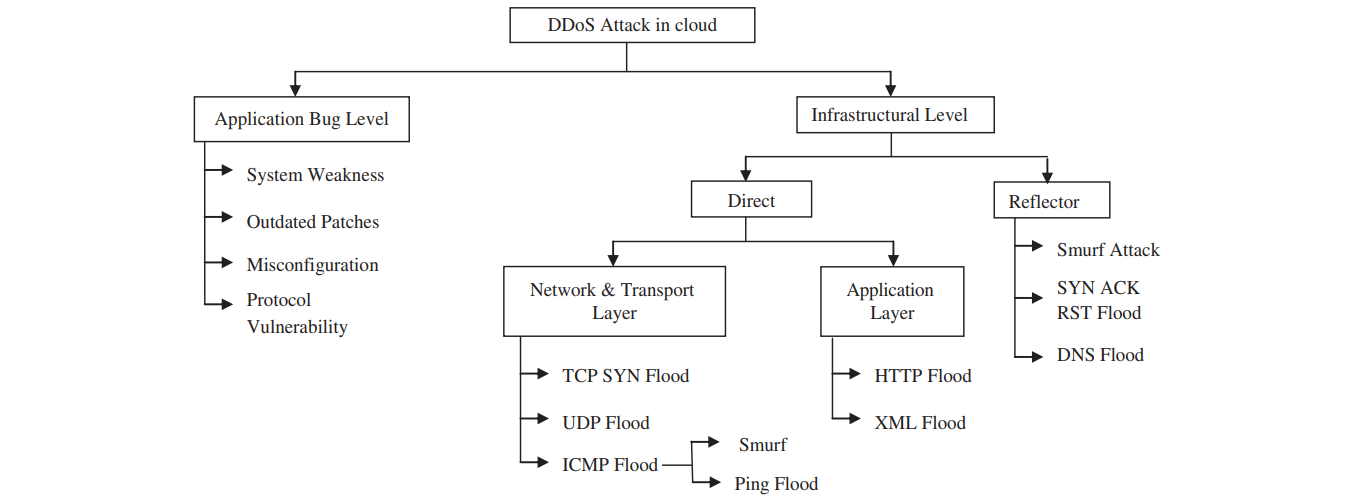
\includegraphics[width=\hsize]{images/introduzione/tipologie_ddos.png}
    \caption{Tipologie di attacchi DDoS}
    \centering
\end{figure}

L'obiettivo di questa sarà concentrato sul rilevamento e la mitigazione della seconda categoria di attacchi, basata sull'esaurimento delle risorse.

\subsubsection{Attacchi basati sul flooding}

TODO

\subsection{Vittime attacchi DDoS}

I target degli attacchi DDoS possono variare molto da un utente domestico ad un governo \cite{ddos_motivations}.

% todo: introduzione: qua potrei nominare delle statistiche sugli attacchi con la distribuzione delle vittime

Per capire maggiormente chi possono essere le vittime di un attacco bisogna analizzare le motivazioni che spingono gli attaccanti e con le diverse motivazioni può cambiare anche la portata dell'attacco. Per semplicità possiamo dividere gli incentivi di un attacco in cinque principali categorie \cite{ddos_survey_1}\cite{ddos_motivations}:

\begin{itemize}
    \item Beneficio economico o finanziario: sono gli attacchi che riguardano principalmente le aziende, sono considerati i più pericolosi e difficili da fermare, perché mirano ad ottenere benefici finanziari dagli attacchi. I creatori dell'attacco normalmente sono persone con esperienza.
    \item Vendetta: questa Tipologia di attacchi sono mesi in atto da persone, solitamente con uno scarso livello tecnico, a fronte di un'apparente ingiustizia percepita.
    \item Credo ideologico: alcuni attaccanti si trovano ad effettuare attacchi contro degli obiettivi per motivi ideologici. È una motivazione di attacco meno comune delle altre, ma può portare ad attacchi di grande entità. % todo: valutare se mettere esempi attacchi tipo cnn 2008, wikileaks 2010 e iran 2009
    \item Sfida intellettuale: gli utenti che sviluppano attacchi per questa motivazione che vogliono imparare e sperimentare a lanciare attacchi, spesso sono giovani appassionati di hacking che grazie alla facilità con cui si possono affittare botnets o utilizzare semplici tool riescono ad effettuare con successo DDoS.
    \item Cyberwarfare: gli attaccanti di questa categoria appartengono ad organizzazioni terroristiche o militari di un paese e sono politicamente motivati ad attaccare risorse critiche di un altro paese. Un grande numero di risorse viene usato per questa tipologia di attacco e può paralizzare le infrastrutture critiche di un paese, portando ad un grave impatto economico.
\end{itemize}


\subsection{Diffusione attacchi DDoS}



\section{Organizzazione della tesi}
